\section{Yard\-Database Class Reference}
\label{classYardDatabase}\index{YardDatabase@{YardDatabase}}
{\tt \#include $<$ys\_\-database.h$>$}

Collaboration diagram for Yard\-Database:\begin{figure}[H]
\begin{center}
\leavevmode
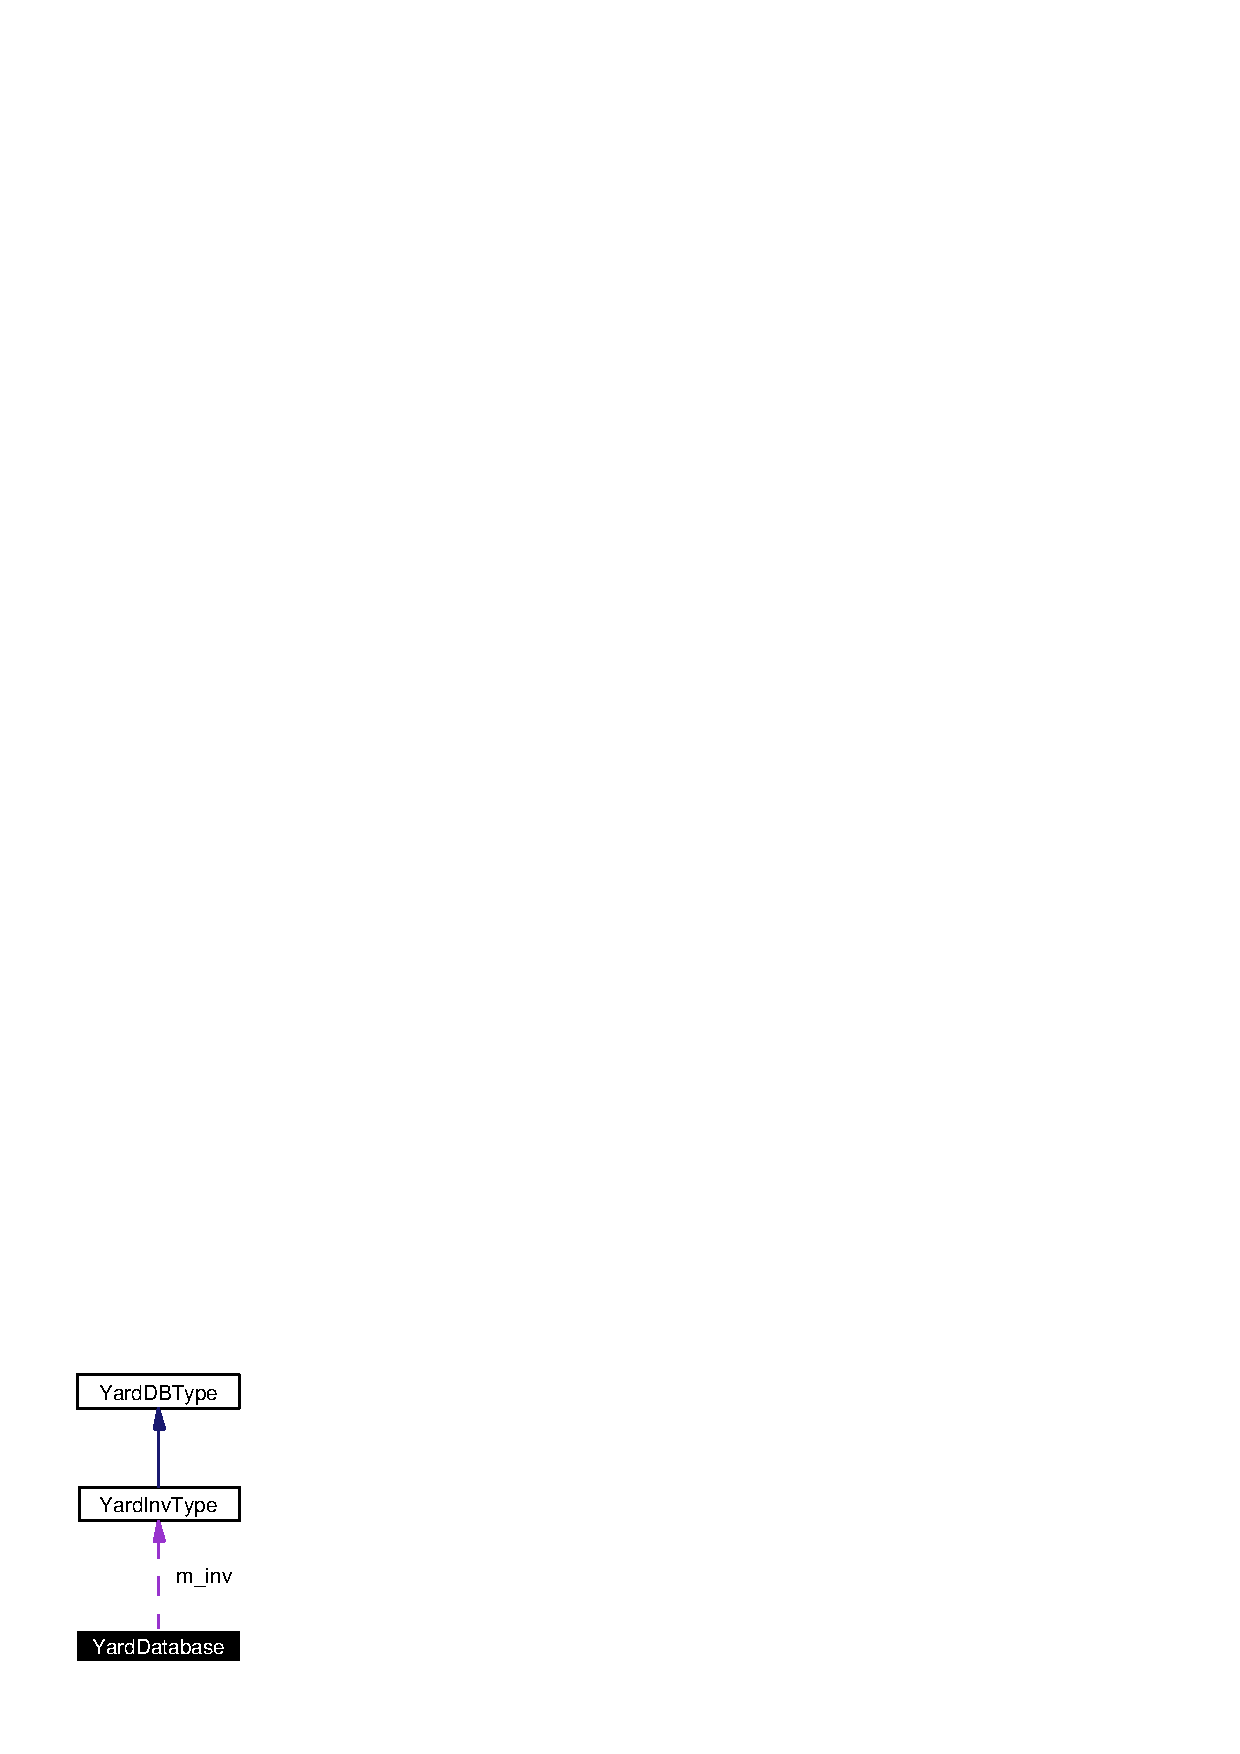
\includegraphics[width=60pt]{classYardDatabase__coll__graph}
\end{center}
\end{figure}


\subsection{Detailed Description}
This is the main database backend which does all translation from OO calls to SQL/ODBC. 

\begin{Desc}
\item[See also:]{\bf Yard\-Inv\-Type}{\rm (p.\,\pageref{classYardInvType})} \end{Desc}


\subsection*{Public Member Functions}
\begin{CompactItemize}
\item 
{\bf Yard\-Database} (const wx\-String \&dsn, const wx\-String \&name, const wx\-String \&pass)\label{classYardDatabase_a0}

\item 
bool {\bf connect} ()\label{classYardDatabase_a2}

\item 
vector$<$ {\bf Yard\-Inv\-Type} $>$ {\bf Inv\-Search\-Keyword} (const unsigned long \&sku)
\begin{CompactList}\small\item\em Find all inventory matches of keyword search. \item\end{CompactList}\item 
vector$<$ {\bf Yard\-Inv\-Type} $>$ {\bf Inv\-Get} (unsigned int num, unsigned int offset)
\begin{CompactList}\small\item\em Get a batch of inventory items. \item\end{CompactList}\end{CompactItemize}


\subsection{Member Function Documentation}
\index{YardDatabase@{Yard\-Database}!InvGet@{InvGet}}
\index{InvGet@{InvGet}!YardDatabase@{Yard\-Database}}
\subsubsection{\setlength{\rightskip}{0pt plus 5cm}vector$<${\bf Yard\-Inv\-Type}$>$ Yard\-Database::Inv\-Get (unsigned int {\em num}, unsigned int {\em offset})}\label{classYardDatabase_a4}


Get a batch of inventory items. 

\begin{Desc}
\item[Parameters:]
\begin{description}
\item[{\em num}]The number of items to get. \item[{\em offset}]The item index to start at. \end{description}
\end{Desc}
\begin{Desc}
\item[Returns:]A std::vector of {\bf Yard\-Inv\-Type}{\rm (p.\,\pageref{classYardInvType})} objects \end{Desc}
\index{YardDatabase@{Yard\-Database}!InvSearchKeyword@{InvSearchKeyword}}
\index{InvSearchKeyword@{InvSearchKeyword}!YardDatabase@{Yard\-Database}}
\subsubsection{\setlength{\rightskip}{0pt plus 5cm}vector$<${\bf Yard\-Inv\-Type}$>$ Yard\-Database::Inv\-Search\-Keyword (const unsigned long \& {\em sku})}\label{classYardDatabase_a3}


Find all inventory matches of keyword search. 

\begin{Desc}
\item[Note:]This could be dangerous, need to limit all returns to some set value (or configured value). \end{Desc}
\begin{Desc}
\item[Parameters:]
\begin{description}
\item[{\em keyword}]A text string to search for. \end{description}
\end{Desc}
\begin{Desc}
\item[Returns:]A std::vector of {\bf Yard\-Inv\-Type}{\rm (p.\,\pageref{classYardInvType})} objects \end{Desc}


The documentation for this class was generated from the following files:\begin{CompactItemize}
\item 
ys\_\-database.h\item 
ys\_\-database.cpp\end{CompactItemize}
